\textbf{Актуальность исследования:}

Компьютеризация и информатизация различных сфер общества и производства неизменно
сопровождается созданием специализированных программных и аппаратных средств.

\begin{figure}[!htbp]
    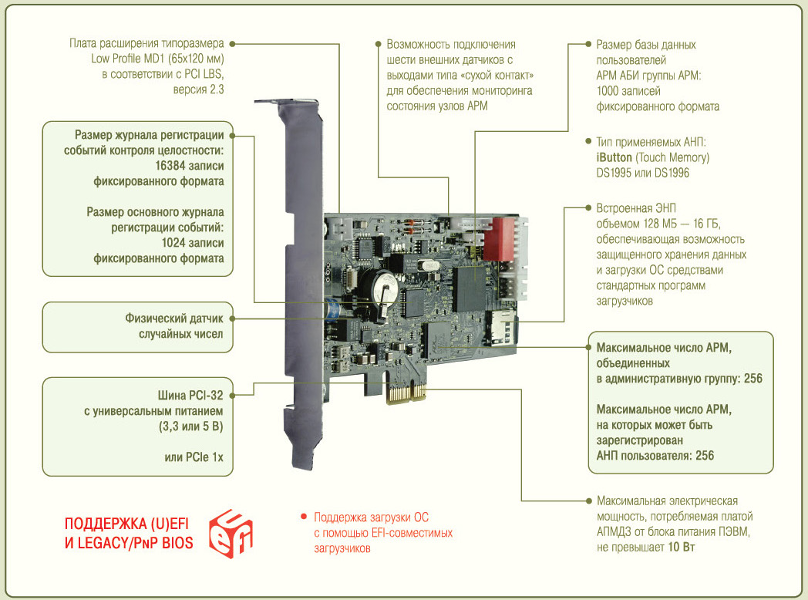
\includegraphics[width=\textwidth,height=\textheight,keepaspectratio]{images/apmdz.png}
    \caption{Пример специализированного аппаратного обеспечения: АПМДЗ Максим-М1\label{fig:apmdz}}
\end{figure}

Разработка аппаратного обеспечения практически никогда не обходится без создания
прикладного програмного обеспечения.
Правильное проектирование архитектуры ПО и выделение уровней абстракции позволяет
разрабатывать программное обеспечение и аппаратное обеспечение параллельно, но
до определенного уровня.

В теории теория и практика не различаются, но не на практике.
Для тестирования и отладки прикладного ПО в конечном счете понадобится аппаратное обеспечение,
но зачастую им сложно обеспечить всю команду разработчиков, особенно на ранних стадиях.
Причиной этому могут быть экономические, логистические, производственные или временные проблемы.

В связи с введением санкций против Российской Федерации, затрагивающих
в том числе и сферу высоких технологий, вероятен срыв цепочек поставок,
ограниченость или невозможность произвести в нужном объеме собственные
аналоги заграничных устройств.
Даннные факторы являются серьезным риском как для высокотехнологических
компаний страны, так и для пользователей их продукции.

Но даже если обеспечить всех разработчиков необходимыми стендами, то при проявлении
проблем во взаимодействии ПО и АО, аппаратное обеспечение придется отправлять на доработку,
после чего снова печатать, доставлять и собирать стенды, что неизбежно приводит к экономическим
и временным издержкам, которые, в свою очередь, повышают затраты на завершение проекта в срок.

Исправить и запустить ПО на поздних этапах проектирования легче, чем исправить и перевыпустить схему.

\textbf{Причины сложившейся ситуации:}

В основном разработкой решений для виртуализации занимаются либо крупные компании вроде VMware, производящие
проприетарное ПО, либо группы энтузиастов, разрабатывающие ПО с открытым исходным кодом, которое
тоже поддерживаются коммерческими компаниями как Red Hat. Поддержка специфических аппаратных решений
ложится на плечи разработчиков этих самых аппаратных решений. Отсутствие необходимой квалификации,
сжатые сроки, потребность в изучении документации по встраиванию виртуальных устройств в существующую
инфраструктуру делают маловероятным и экономически необоснованным выделение времени и
человеческих ресурсов на создание эмуляторов проектируемого аппаратного обеспечения.

\textbf{Необходимость создания методики и алгоритма генерации виртуального аппаратного
обеспечения по спецификации:}

Отсутствие быстрого способа создания эмуляторов специализированного аппаратного обеспечения, что отражается
экономических аспектах конечного продукта.

\textbf{Новизна исследования:}

Технологии и подходы к эмуляции аппаратного обеспечения используются давно,
но на данный момент существует лишь один инструмент \cite{imposters}, который позволял
бы быстро и просто создавать эмуляторы любых аппаратных устройств.


\textbf{Значимость:}

Данная работа стремится улучшить пользовательский опыт в области разработки эмуляторов
аппаратного обеспечения и развить идеи имеющихся программных решений в данной области,
повысив тем самым скорость, надежность и простоту разработки эмуляторов устройств.
